% Requires: graphicx, booktabs, amsmath
\subsection{One-Dimensional Allen--Cahn Equation}
\label{subsec:ac-onestep}

We consider the one-dimensional Allen--Cahn equation
\begin{equation}
\frac{\partial u}{\partial t} - 10^{-4} \frac{\partial^2 u}{\partial x^2} + 5\left(u^3-u\right) = 0,
\qquad (x,t)\in[-1,1]\times(0,1],
\label{eq:ac-governing}
\end{equation}
with the initial condition
\begin{equation}
u(x,0)=x^2\cos(\pi x),
\label{eq:ac-initial}
\end{equation}
and periodic boundary condition
\begin{equation}
u(-1,t)=u(1,t).
\label{eq:ac-periodic}
\end{equation}
The reference solution is taken from the high-resolution Chebfun dataset stored in the current repository. All cases reported in this subsection are the actual regression cases under
\texttt{cases/nonlinear\_pde\_cases/time\_pde\_cases/Allen\_Cahn/}, so the numerical settings below are consistent with the executable benchmarks rather than post hoc hand-tuned descriptions.

\paragraph{One-step predictor--corrector time discretization.}
The default time integrator for the time-dependent nonlinear PDE solver is the \texttt{onestep\_predictor} scheme. In the general framework, it is written as
\begin{equation}
\frac{u^{*}-u^{n}}{\Delta t} + \mathcal{L}_{1}(u^{*})
 + \mathcal{L}_{2}(u^{*})\,F(u^{n}) + \mathcal{N}(u^{n}) = 0,
\label{eq:onestep-predictor}
\end{equation}
followed by the explicit corrector
\begin{equation}
u^{n+1}
=
u^{n}
- \Delta t
\left[
\overline{\mathcal{L}_{1}\beta}
+
\overline{\mathcal{L}_{2}\beta}\,F(u^{n+\frac12})
+
\mathcal{N}(u^{n+\frac12})
\right],
\label{eq:onestep-corrector}
\end{equation}
where
\begin{equation}
u^{n+\frac12}=\frac{1}{2}\left(u^{n}+u^{*}\right).
\label{eq:onestep-midpoint}
\end{equation}
The implementation uses operator reuse between consecutive steps, so the linear operator contributions in the corrector are averaged from the previous and current predictor evaluations. In addition, the first predictor step uses a reduced time increment $0.1\Delta t$ to suppress start-up transients, and the corrector is activated from the second full step onward.

For the Allen--Cahn case in \eqref{eq:ac-governing}, $\mathcal{L}_{2}=0$, and thus \eqref{eq:onestep-predictor} simplifies to
\begin{equation}
\frac{u^{*}-u^{n}}{\Delta t} - 10^{-4}u^{*}_{xx} + 5\left[(u^{n})^3-u^{n}\right] = 0,
\label{eq:ac-predictor}
\end{equation}
while the corrector reduces to a midpoint update with the nonlinear reaction term evaluated at $u^{n+1/2}$. This design is particularly effective for the present benchmark because the stiff diffusion contribution is treated implicitly in the predictor, whereas the nonlinear term is advanced with a low-cost explicit correction.

\paragraph{Numerical configuration.}
Unless otherwise stated, all Allen--Cahn runs in this subsection use the same neural architecture
\texttt{[12, 32, 32, 10]}, polynomial degree $10$, periodic boundary pairing with one constraint point, one swap point per step, $20{,}000$ Adam iterations for each spotter call, and no L-BFGS phase. The scalar solution is represented on segmented polynomial patches, where the segment count is varied to study the trade-off between locality and cost. Error statistics are taken from each case's \texttt{error\_statistics\_report.txt}. For the \texttt{onestep\_predictor} cases, the reported errors are evaluated from the prediction exported on the case grid, not from an isolated single-time snapshot.

\begin{figure}[t]
    \centering
    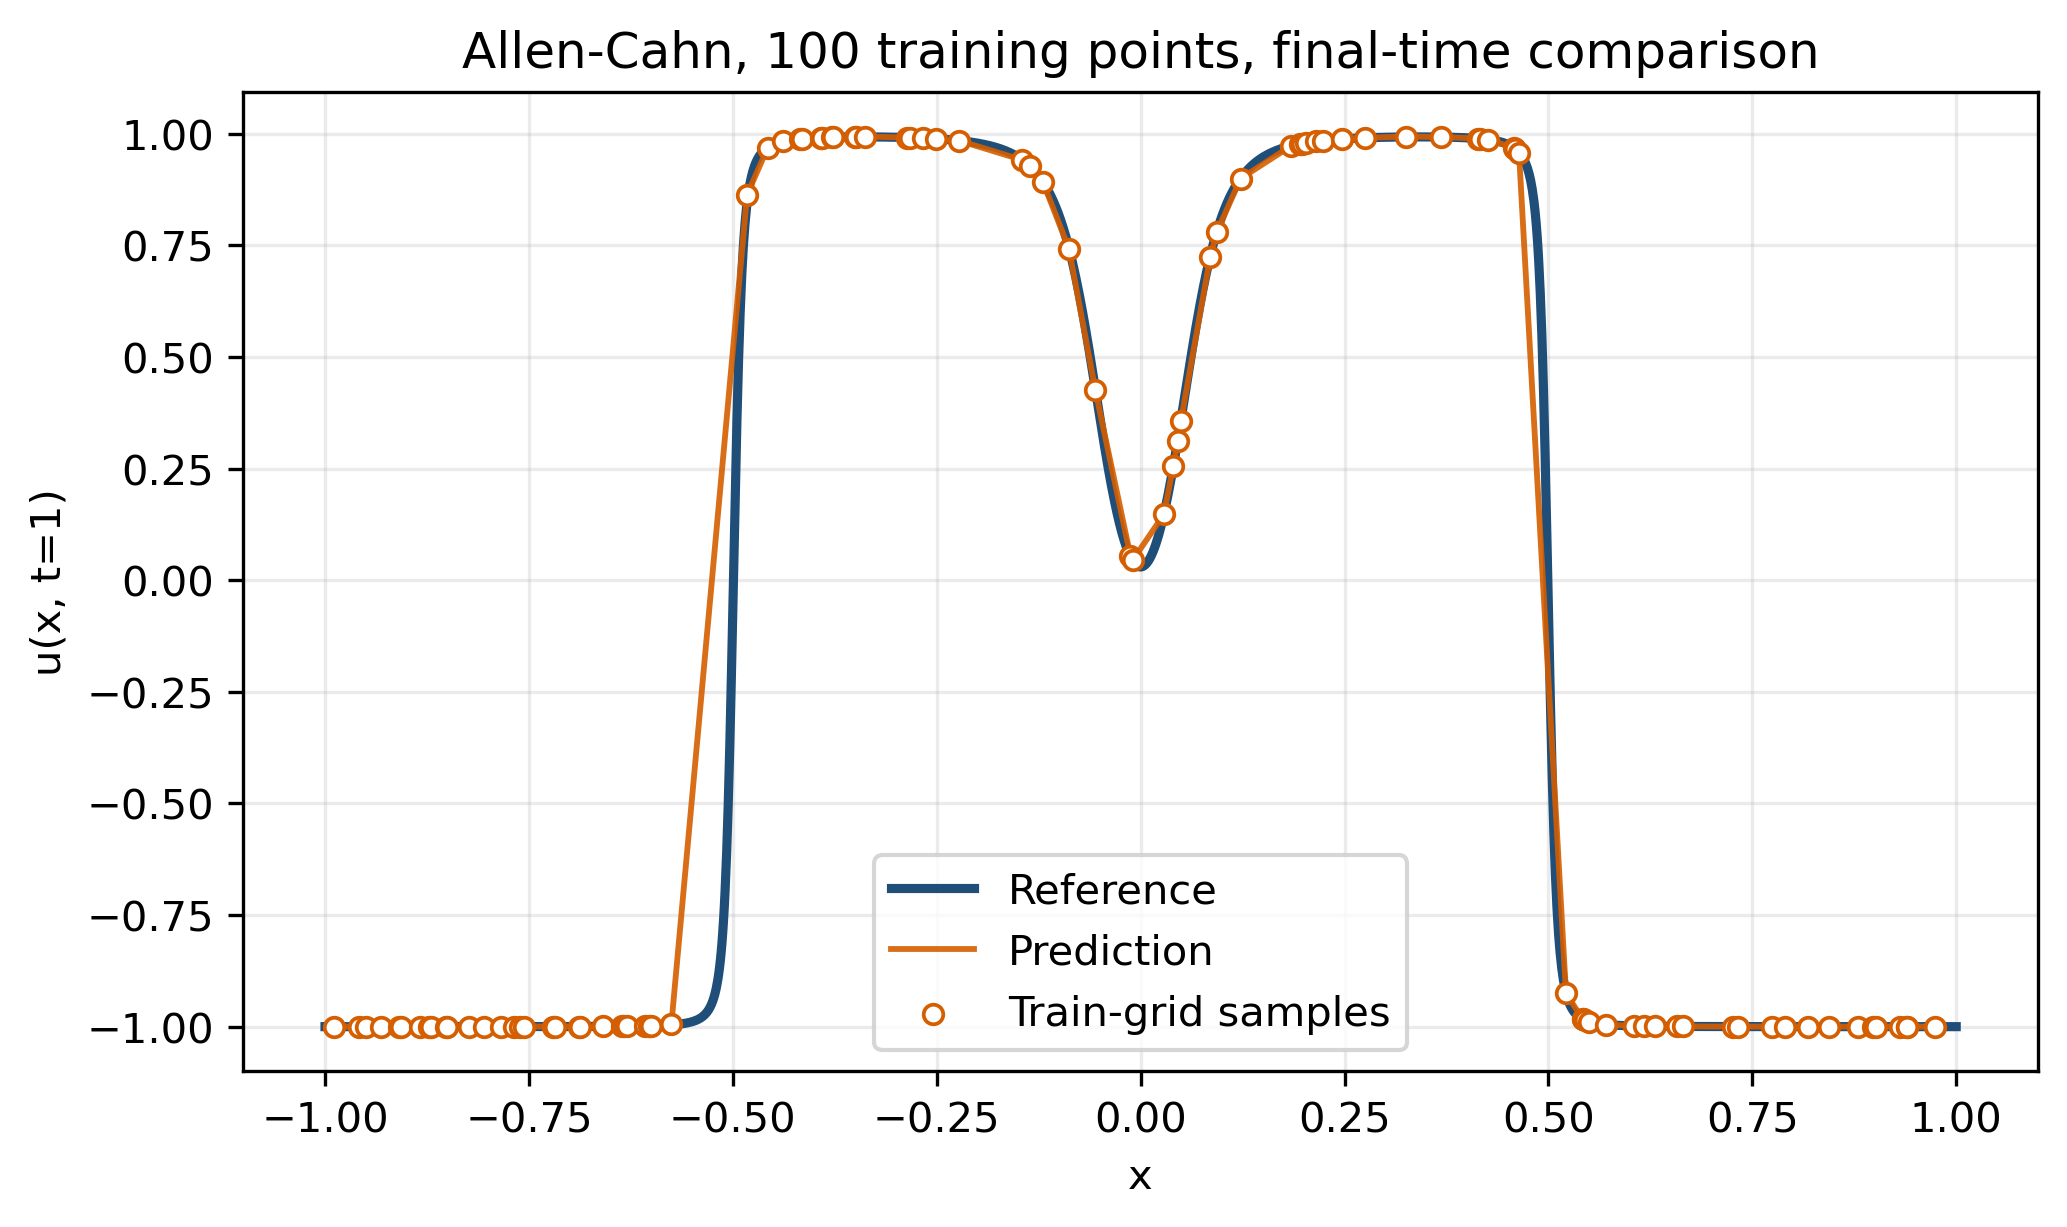
\includegraphics[width=0.72\linewidth]{figures/ac_100pts_train_scatter_final.png}
    \caption{Final-time solution comparison for the $100$-point Allen--Cahn benchmark with $\Delta t=0.01$. The markers are the training-grid scatter points, and the curves show the reference and predicted solutions. Even with only $100$ spatial points, the solution profile is already captured accurately.}
    \label{fig:ac-100pts-scatter}
\end{figure}

\begin{table}[t]
    \centering
    \caption{Regression results of five one-step predictor Allen--Cahn benchmarks.}
    \label{tab:ac-onestep-five-cases}
    \resizebox{\linewidth}{!}{%
    \begin{tabular}{lcccccccc}
        \toprule
        Case & Points & Segments & $\Delta t$ & Steps & Global $L_2$ & Time-average $L_2$ & Max $L_2$ & Time (s) \\
        \midrule
        \texttt{AC\_equation\_100\_0.1} & 100 & 3 & 0.1   & 11  & $2.271687\times10^{-2}$ & $2.104173\times10^{-2}$ & $3.199721\times10^{-2}$ & 2.77 \\
        \texttt{AC\_equation\_100\_0.01} & 100 & 3 & 0.01  & 101 & $6.891622\times10^{-4}$ & $6.103482\times10^{-4}$ & $1.868757\times10^{-3}$ & 9.00 \\
        \texttt{AC\_equation\_500\_0.05} & 500 & 10 & 0.05  & 21  & $6.720012\times10^{-3}$ & $6.294634\times10^{-3}$ & $9.382784\times10^{-3}$ & 6.51 \\
        \texttt{AC\_equation\_500\_0.01} & 500 & 10 & 0.01  & 101 & $3.189989\times10^{-4}$ & $3.026821\times10^{-4}$ & $4.406851\times10^{-4}$ & 20.84 \\
        \texttt{AC\_equation\_500\_0.005\_20seg} & 500 & 20 & 0.005 & 201 & $3.084215\times10^{-4}$ & $1.399946\times10^{-4}$ & $2.214110\times10^{-3}$ & 62.07 \\
        \bottomrule
    \end{tabular}}
\end{table}

Table~\ref{tab:ac-onestep-five-cases} shows three clear trends. First, the $100$-point configuration is already competitive: reducing the time step from $0.1$ to $0.01$ lowers the global $L_2$ error from $2.27\times10^{-2}$ to $6.89\times10^{-4}$, while the total physical solve time remains only $9$ seconds. This makes the $100$-point case a useful efficiency-oriented configuration rather than a mere toy example. Second, increasing the spatial points from $100$ to $500$ and reducing $\Delta t$ from $0.05$ to $0.01$ further lowers the global error to $3.19\times10^{-4}$ with a still modest runtime of $20.84$ seconds. Third, increasing the segment count from $10$ to $20$ together with a smaller time step $\Delta t=0.005$ gives the best mean behavior, reducing the time-average $L_2$ error to $1.40\times10^{-4}$.

However, the improvement is not uniform across all metrics. The most accurate average case,
\texttt{AC\_equation\_500\_0.005\_20seg}, also exhibits a larger maximum-in-time $L_2$ error and a noticeably larger global $L_\infty$ error than the more balanced
\texttt{AC\_equation\_500\_0.01} configuration. This indicates that once the Allen--Cahn interface enters its late-time steeper-gradient regime, the residual error becomes increasingly dominated by the spotter fitting stage rather than the formal first-order predictor discretization alone. In other words, smaller $\Delta t$ and more segments continue to improve the average trajectory, but they do not guarantee monotonic improvement of the worst-time local error. This limitation should be stated explicitly when discussing accuracy saturation for phase-field dynamics with evolving sharp fronts.

\paragraph{Comparison with existing PINN literature.}
Representative Allen--Cahn PINN studies include adaptive PINN domain treatment \cite{wight2021adaptive}, sequential time-slab training \cite{mattey2022sequential}, hard-constraint wide-body PINNs \cite{chen2024hwpinn}, and more recent dual-level time-marching neural networks \cite{guo2025dualtime}. Among the papers that explicitly report both accuracy and runtime for a one-dimensional Allen--Cahn benchmark, Chen et al.~\cite{chen2024hwpinn} reported a relative $L_2$ error of $7.10\%$ and a computational time of $1654$ s for their HWPINN model, while Grossmann et al.~\cite{grossmann2024fem} concluded from a broader computational study that PINNs did not outperform FEM in either solution time or accuracy on the tested problems, including $1$D Allen--Cahn. These comparisons are not strictly apples-to-apples because the PDE parameterization, hardware, norm definition, and reference discretization differ across studies. Nevertheless, they still provide two useful messages: time-dependent phase-field problems remain challenging for monolithic PINN training, and temporal-marching formulations are generally more favorable than a single global space-time fit. The behavior observed in Table~\ref{tab:ac-onestep-five-cases} is consistent with this literature trend.

\paragraph{Summary of the benchmark.}
Overall, this Allen--Cahn benchmark is an efficient regression case for the current framework. The full solver remains fast at low to medium point counts, and the $100$-point benchmark already attains a fairly high accuracy with a short wall-clock time. As the number of spatial points increases, the segment count is refined, and the time step is reduced, the average accuracy improves clearly. At the same time, because the late-time solution develops stronger gradients and the spotter stage becomes dominant, the peak error does not improve as smoothly as the average error. This makes the benchmark a useful test for both efficiency and robustness: it is cheap enough for routine regression, yet still rich enough to reveal the accuracy bottleneck of the current spotter-dominated phase in the steep-gradient regime.
